\documentclass[aspectratio=169]{beamer}
\usetheme{Madrid}
\usepackage[T1]{fontenc}
\usepackage[utf8]{inputenc}
\usepackage[spanish,es-nodecimaldot]{babel}
\usepackage{amsmath}
\usepackage{booktabs}
\usepackage{graphicx}
\usepackage{siunitx}
\DeclareSIUnit\mmHg{mmHg}

\title{Proyecto AASIM}
\subtitle{Estimación Continua de Presión Arterial vía ECG}
\author{Equipo E (Juan Manuel Buitrago, Luis Carlos Rocha, German Alberto Hidalgo)}
\date{\today}

\begin{document}

\begin{frame}
  \titlepage
\end{frame}

\begin{frame}{Problema y arquitectura}
  \textbf{Problema:} los monitores de presión arterial de manguito generan
  ``puntos ciegos clínicos'' que impiden anticipar crisis hipertensivas.

  \vspace{0.5em}
  \textbf{Estructura PICO}
  \begin{itemize}
    \item \textbf{P:} Adultos con registros simultáneos de ECG y presión arterial.
    \item \textbf{I:} SaMD con Machine Learning sobre el ECG continuo para predecir PAS, PAD y PAM.
    \item \textbf{C:} Esfigmomanómetros electrónicos validados (\textit{ground truth}).
    \item \textbf{O:} MAE, RMSE y \% de predicciones en rango clínicamente aceptable.
    \item \textbf{T:} Ventanas de adquisición de 30 s a 5 min.
  \end{itemize}
\end{frame}

\begin{frame}{Métodos y validación}
  \textbf{Estrategia de datos}
  \begin{itemize}
    \item Extracción de características (p. ej. HRV) controlando confusores: edad, sexo, medicamentos, postura.
    \item Particiones sin fuga de datos: un mismo paciente no aparece en entrenamiento y validación/prueba.
    \item \textbf{Baseline:} regresión lineal sobre el Tiempo de Tránsito del Pulso (PTT).
    \item \textbf{SOTA:} arquitecturas de Deep Learning para bioseñales, usadas como comparación.
  \end{itemize}

  \vspace{0.5em}
  \textbf{Criterios de éxito}
  \begin{table}
    \centering
    \begin{tabular}{llc}
      \toprule
      Tipo & Métrica & Umbral \\
      \midrule
      Primaria & MAE PAS/PAD & $\le 5$ \si{\mmHg} \\
      Primaria & RMSE & $\le 8$ \si{\mmHg} \\
      Secundaria & Correlación (r) & $\ge 0.85$ \\
      Técnica & Latencia de inferencia & $\le 5$ s \\
      \bottomrule
    \end{tabular}
  \end{table}
\end{frame}

\begin{frame}{Resultados}
  \centering
  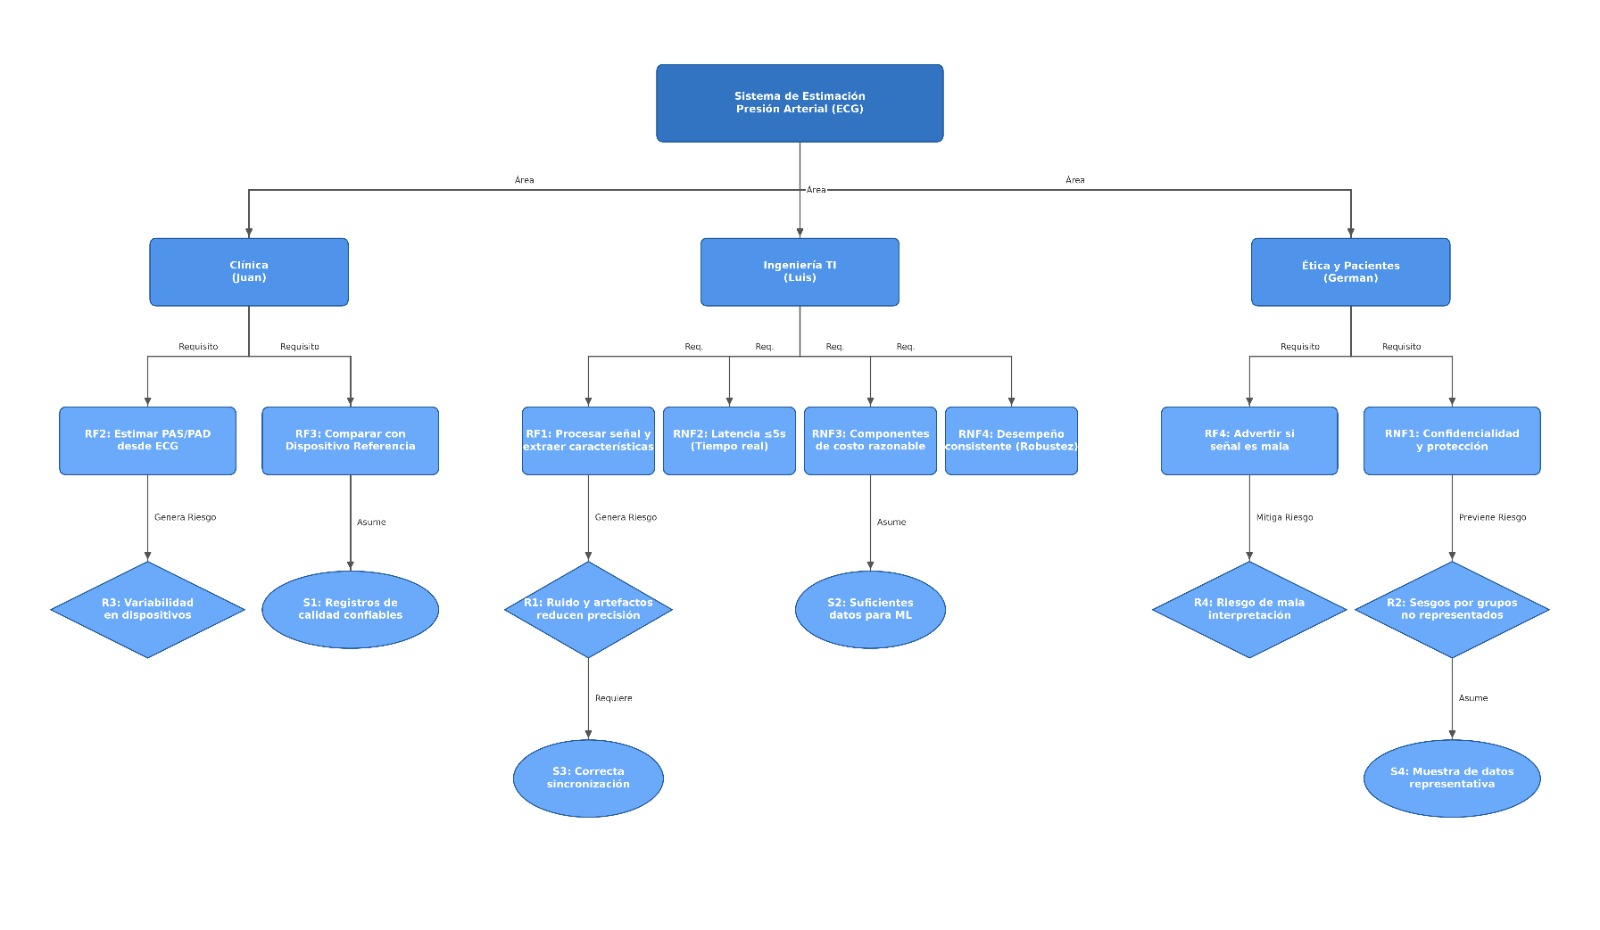
\includegraphics[width=0.88\linewidth]{figures/summary.png}
\end{frame}

\begin{frame}{Reproducibilidad y limitaciones}
  \begin{itemize}
    \item \textbf{Evaluación por subgrupos:} métricas desglosadas por edad, sexo y comorbilidades para mitigar sesgos algorítmicos (Riesgo R2).
    \item \textbf{Privacidad:} anonimización irreversible de registros fisiológicos antes del pipeline de TI (RNF1).
    \item \textbf{Control de calidad de señal:} si el ECG presenta ruido excesivo, el sistema omite la predicción en vez de generar falsos positivos (RF4).
    \item \textbf{Alcance:} resultados válidos dentro de las ventanas y poblaciones definidas en el PICO; no sustituye el diagnóstico clínico.
  \end{itemize}
\end{frame}

\end{document}
